\chapter{SleeveAR}
\label{sec:sleevear}

%\section*{Summary}

This chapter describes a new approach to deal with the various SleeveAR implementation challenges, and  identifies the critical resources required for a successful implementation. It is presented the design options for providing the visual and audio feedback information.

\todo{Artur: "establish the most important requirements and objectives to be achieved by the solution" - isto deve ser feito logo na intro, em Requirements and Goals, e não aqui.}


\section{Approach}
\label{sec:sleevear:approach}

\begin{figure}[!t]
    \begin{center}
        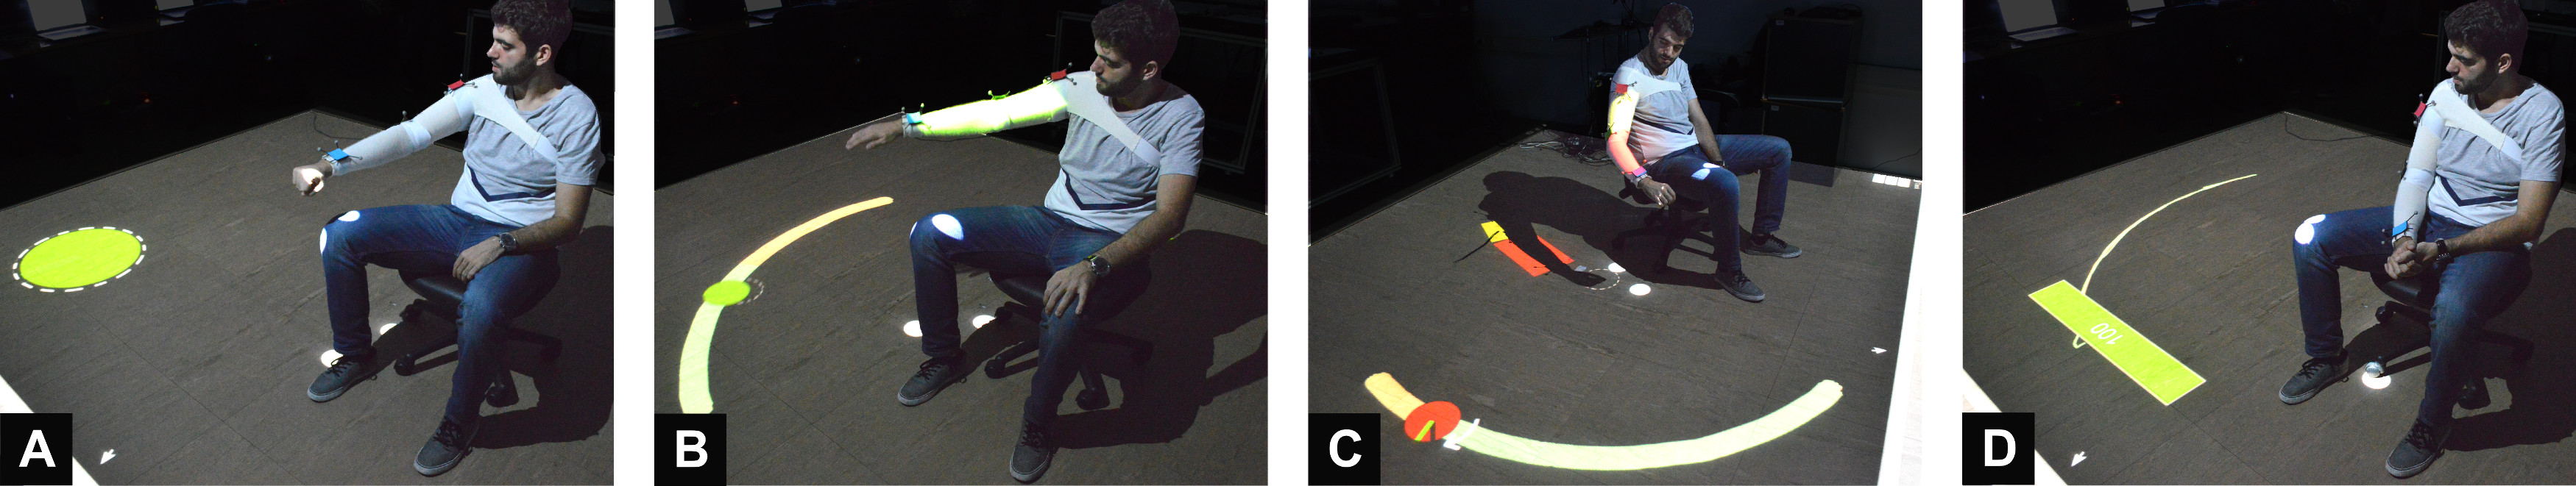
\includegraphics[width=\textwidth]{imgs/impl/teaser.jpg}
    \end{center}
    \caption{SleeveAR addresses new active projection-based strategies for providing user feedback during rehabilitation exercises. a) Initial position. b) Mid-performance. c) Sleeve Feedback. d) Performance review.}
    \label{fig:teaser}
\end{figure}

SleeveAR has ambitious goals, aiming further beyond the accomplishments achieved by LightGuide. 
As described in the previous section, LightGuide only focused on projecting information on top of the hand. Not only does this leaves a small room for movement diversity, but also reduces the amount of possible and useful information that can be given.
By increasing the projection area throughout the whole arm and user's surrounding environment areas, we can successfully improve an user's awareness while a movement is being executed. 
\todo{em vez de 'not only that, blah blah blah, ser por ex. "IN ADDITION, if it was possible for the movement THAT IS being replicated to be...} Not only that, but if it was possible for the movement being replicated to be originated by another person, we could achieve a much more realistic and useful guidance.
With SleeveAR, virtual content can be projected onto different surfaces, and even, onto people's own limbs, to provide, in real-time, a more immersing experience. 

Our vision consists of the possibility of recording exercises by demonstration. From there, our approach should guide other users in their attempt to recreate them based on the recording made.
SleeveAR should follow a specific process in his implementation, which will be explained in the section.

%consists of two main concepts. Firstly, the precise recording of the exercise being demonstrated by a personal therapist. 
%And secondly, the ability to properly guide another person, the rehabilitation subject, during the execution of the pre-recorded exercise.
%Hereafter we will describe in detail each of this general concepts of our vision.

%While, at the same time, provide awareness of the rehabilitation exercise progress to insure the correctness of the patient's movements.
%With SleeveAR, a therapist can easily demonstrate the prescribed exercises and make sure his patient will perform them correctly without the requirement of his close supervision.

%In the SleeveAR system, the exercise being performed needs to be recorded beforehand, which, in this case, should be a health professional. 
%Not only it provides a great range of possible movements, but also assigns,onto the professional, the responsibility of providing adequate exercises based on a specific patient's condition.




\section{Process (Or SleeveAR Workflow)}

\todo{referenciar a imagem do teaser aqui}

The SleeveAR process can be divided into three main phases. 
The first one, \textbf{Recording}, involves someone demonstrating an exercise so it can be recorded by SleeveAR. 
Next, we have the \textbf{Movement Guidance} phase, which focus on guiding another person in order to recreate the previously recorded exercise.
Our final phase, \textbf{Performance Review}, should provide the user with an evaluation of his performance, by comparing with the original exercise.
Each of this phases will be individually described in the following sections.

\begin{figure}[!h]
    \begin{center}
        
\includegraphics[width=0.6\textwidth]{imgs/approach/sleevear-progress}
    \end{center}
    \caption{Upper Arm Visual Feedback.}
    \label{fig:upperarmfeedback}
\end{figure}

\subsection{Recording}

Usually, the patient's prescribed exercises were specifically conceived for the current patient's health condition. 
With this in mind, we wanted to maintain this relation between a therapist and a patient, by giving the therapists the power for demonstrating the prescribed exercises to the patient. 
Based on this demonstration, SleeveAr will capture the therapist movement, and it will build and store its model for a later usage.
By giving the therapist the responsibility of demonstrating the exercise, we do not need to worry about the physical limitations of the patient that would use our system to recreate it. 
We are assuming the recorded exercise is already customized for the patient in question.

Given these assumptions, SleeveAr must then be able to guide a patient through those exercises as best as possible. Hence, we will now describe the SleeveAR's intended behaviour for guiding a patient.


\subsection{Movement Guidance}
Our approach divides the task for guiding a patient through
an exercise into two steps, reaching the first
initial position of  the  exercise, see  Figure~\ref{fig:teaser}A,  and exercise performance, see  Figure~\ref{fig:teaser}B. 

These steps constitute a simple and clear process for organizing the desired actions to be performed by SleeveAR while interacting with a patient.
To successfully recreate an exercise, we considered the user must first reach the exercise initial position, i.e., the first arm position from the recorded demonstration.
For accomplishing this first task, as shown in Figure~\ref{fig:teaser} A), a patient must follow SleeveAR's feedback to achieve the correct arm position (such feedback information is explained in Section~\ref{sec:feedback}).
After the initial position has been reached, as determined by SleeveAR, the system starts guiding the user through the remaining exercise.

It could be an almost impossible task for a patient to exactly recreate the original demonstration of the exercise. 
With this in mind, SleeveAR needs to rely on thresholds for specific values of tolerance. 
By doing so, if it were required of a patient to achieve, for example, a 90 degree arm flexion, he would not 
need to actually achieve it, being only enough for him to get close to that degree of flexion according to the specified tolerance.
In figure~\ref{fig:teaser} B) and C), we see two examples where the user is being guided corrected in case it was necessary.


\subsection{Performance Review}

\begin{figure}
    \begin{center}
        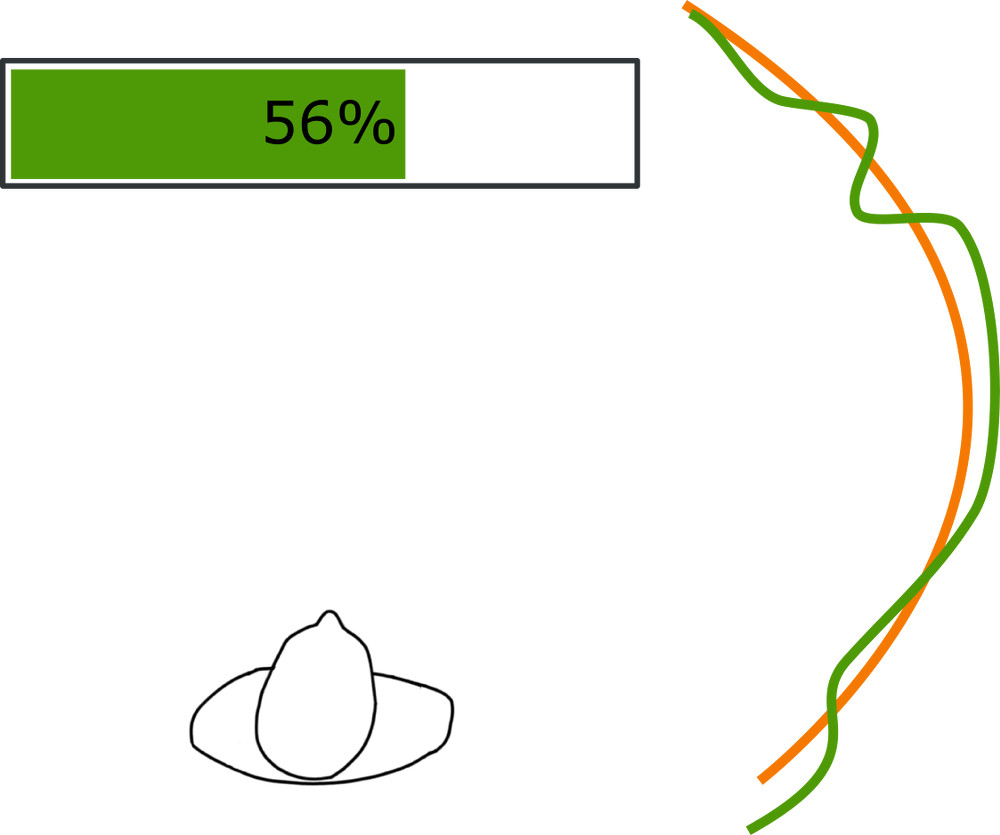
\includegraphics[width=0.35\textwidth]{imgs/approach/performancereview}
    \end{center}
    \caption{Performance Review.}
    \label{fig:performancereview}
\end{figure}

At the end of each exercise, SleeveAR should provide an overview of the patient's performance in comparison with the original, seen at figure \ref{fig:teaser} D).
This will help the patient understand what he might have done wrong and in which parts of the exercise he could still improve his performance.
To successfully guide a patient through his exercises, while informing him of his own performance, we need to plan how SleeveAR should interact with its users. 
Patients will be informed about their performance by two different designs. 
First, and most importantly, the trajectory of the original exercise will be drawn on the floor, followed by the user's recently executed attempt. 
These trajectories will help to visualize what fractions of the exercise could be improved.
The second feedback mechanism consists of computing a score, based on similarity between both movements. This score is also projected on the floor. 
With this small gamification, users will feel motivated to improve their score and, consequently, also improve their overall performance.

Figure \ref{fig:performancereview} provided an example where an orange and green line are drawn on the floor, representing the original trajectory and user's attempt movement trajectory, respectively. 
The calculated score should be shown with a simple horizontal bar, including the calculated percentage of similarity.


\section{Feedback}
\label{sec:feedback}

Several strategies can be followed for the provisioning of feedback to the users. 
Our approach mainly focus on providing visual feedback through the use of light projectors. 
Based on our research, and previous related work, visual feedback is considered to be the most suitable feedback type for spatial information. 
Since our goal was to guide users through physical movements, there is no doubt visual feedback should be the appropriate choice for it.

Audio Feedback was also used, even if with a less vital role compared to visual.
Its was mainly aimed at notifying users about a specific event. In Section~\ref{audio-feedback} we will describe its use in more detail.


\subsection{Visual Feedback}
\label{vision-feedback}


\begin{figure}[!t]
\minipage[t]{0.49\textwidth}
  \centering
  \includegraphics[width=0.7\linewidth]{imgs/approach/elbowangle}
    \caption{Elbow Angle Definition.}
    \label{fig:elbowangle}
    \endminipage\hfill
\minipage[t]{0.49\textwidth}
  \centering
  \includegraphics[width=0.9\linewidth]{imgs/approach/forearmfeedback}
    \caption{Fore Arm Visual Feedback.}
    \label{fig:forearmfeedback}
    \endminipage
\end{figure}



%\begin{figure}[!t]
%    \begin{center}
%        \includegraphics[width=0.5\textwidth]{imgs/elbowangle.png}
%    \end{center}
%    \caption{Elbow Angle Definition.}
%    \label{fig:elbowangle}
%\end{figure}

A useful and minimalist design was targeted for the visual feedback. There were some key points we wanted to address when designing it.
First of all, the visual information had to provide the user with a representation of his \textbf{current} position, while also showing the \textbf{desired} position. 
These representations had to be done in a way the user would easily comprehend what to do for achieving a desired position.
To provide suitable feedback regarding the full arm, we first applied a different design for each of the regions. Next, we will present our planned visual feedback designs.

Our goal with the following feedback was to accomplish a clear correction of the users arm in the context of the several types of anatomic movements an arm can have. 
For each visual feedback described, we will refer to the corresponding anatomic arm movement.

\subsubsection{Fore Arm}

The fore arm feedback addresses two types of anatomic movement, known as \textbf{flexion} and \textbf{extension} of the arm. 
This type of movements affect an angle between two parts of the body, which in this case refers to the angle between the upper and fore arm. 
This specific angle will be denoted as the \textbf{elbow angle}.
With this in mind, the fore arm range of motion could be summarized in extension and flexion of the arm.
Looking at figure \ref{fig:elbowangle}, we can see an example of two different elbow angles. 
On the left, we observe an elbow angle $\theta$$_1$ of approximately 180 degrees, while on the right an elbow angle $\theta$$_2$ of 90 degrees.  
Whenever extending or flexing the arm, if we are essentially changing the elbow angle, then our feedback should focus on this same angle.

As we said previously, we wanted both designs to represent the current and desired state. 
Our final design for a fore arm feedback makes use of a circle with two bars, similar to a clock with two pointers.

%\subsubsection{Current State}

%\begin{figure}[!t]
%    \begin{center}
%        \includegraphics[width=0.5\textwidth]{imgs/forearmfeedback.png}
%    \end{center}
%    \caption{Fore Arm Visual Feedback.}
 %    \label{fig:forearmfeedback}
%\end{figure}

To represent the current state, we use the black bar, seen in figure \ref{fig:forearmfeedback}. Whenever the user moves his fore arm, this bar will move accordingly.
On the other hand, the desired fore arm state is represented by the green bar. 
For the user to achieve this state, he needs to move his fore arm so that the black bar reaches the green bar.

To extend the user's awareness we added two additional features specifically to this design. 
Depending on the distance between both bars, the circle color would fade between red (too far from goal), and green (for close enough). 
In addition, if the black bar gets too far from the desired position, rotating arrows will appear to warn the user that he is currently not correctly positioned. 
Next we present the planned design for the upper arm feedback.

\subsubsection{Upper Arm}


\begin{figure}[!t]
\minipage[t]{0.49\textwidth}
  \centering
  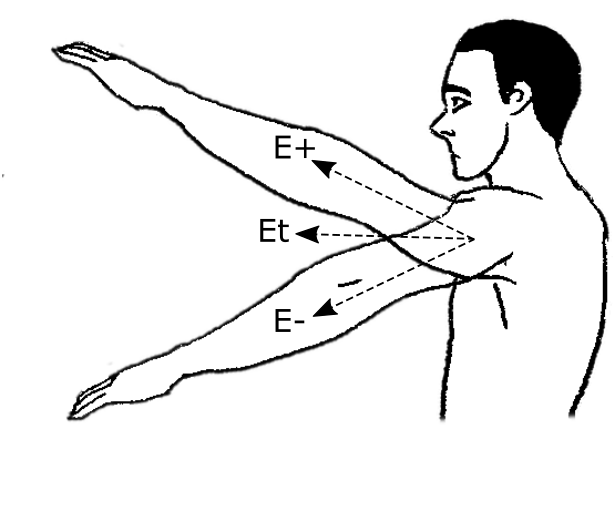
\includegraphics[width=0.8\linewidth]{imgs/approach/elevation_depression}
    \caption{Arm Elevation and Depression.}
    \label{fig:elevation_depression}
    \endminipage\hfill
\minipage[t]{0.49\textwidth}
  \centering
  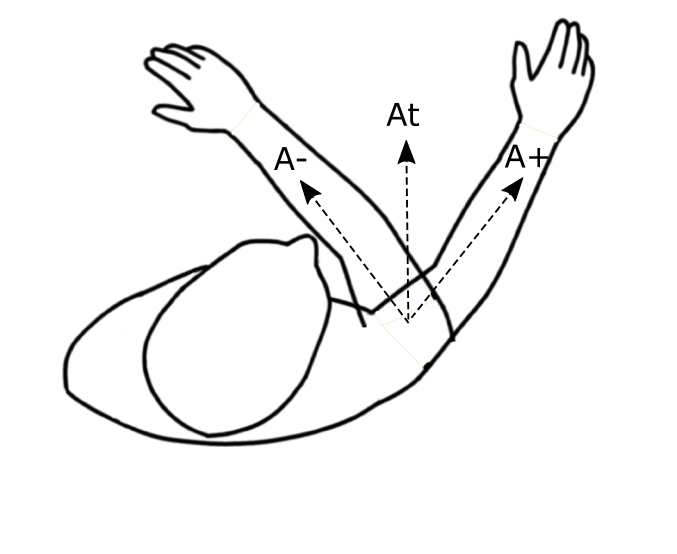
\includegraphics[width=0.8\linewidth]{imgs/approach/abduction_adduction}
    \caption{Arm Abduction and Adduction.}
    \label{fig:abduction_adduction}
    \endminipage
\end{figure}

\begin{figure}[!t]
\minipage[t]{0.49\textwidth}
  \centering
  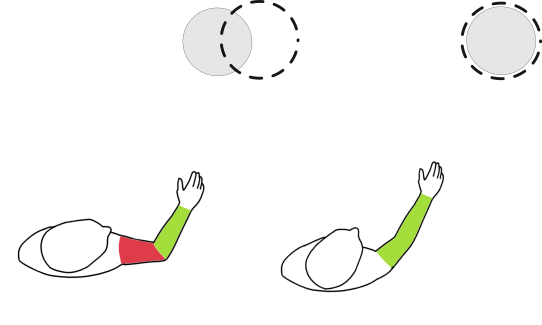
\includegraphics[width=0.8\linewidth]{imgs/approach/upperarmfeedback}
   \caption{Upper Arm Visual Feedback.}
   \label{fig:upperarmfeedback}
    \endminipage\hfill
\minipage[t]{0.49\textwidth}
  \centering
  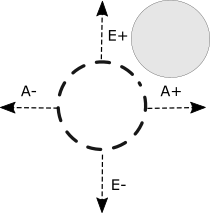
\includegraphics[width=0.5\linewidth]{imgs/approach/upperarmcirclemovement}
    \caption{Dotted circle possible directions.}
    \label{fig:upperarmcirclemovement}
    \endminipage
    \end{figure}

The upper arm movement addresses 4 types of anatomic movements. 
The first two, \textbf{elevation} and \textbf{depression}, represent moving the arm above or below an horizontal line. 
While \textbf{abduction} and \textbf{adduction}, represent moving the arm away from or towards the centre of the body.

Due to these four possible movements being defined by the upper arm direction, we can use this same direction to address all of them. 
The upper arm direction is obtained by a directional vector from the shoulder to the elbow.
In order to facilitate the upper arm feedback understanding, we will consider \textbf{depression} as a negative \textbf{elevation} and \textbf{adduction} as a negative \textbf{abduction}.

Observing the figure \ref{fig:elevation_depression}, we have an example where \textit{Et} represents the elevation target, while, relative to this target, the user could have higher elevation (\textit{E+}) or lower elevation (\textit{E-}).
While in figure \ref{fig:abduction_adduction}, we observe an abduction target, \textit{At}, and following the previous example, higher or lower abduction \textit{A+} and \textit{A-}.

Once again, it was necessary for the design (represented in fig \ref{fig:upperarmfeedback}) to both show the current and desired states. 

%\subsubsection{Current State}

A dotted circumference was chosen to represent the upper arm current state. Moving the upper arm accordingly to the possible movements described in figures \ref{fig:elevation_depression} and \ref{fig:abduction_adduction} will cause the dotted circle to move in a 2D plane respectively. 
In figure \ref{fig:upperarmcirclemovement} we can see the influence of each specific movement has on the dotted circle position. 
It should also be stated that there is nothing impeding a combination of both elevation and abduction movements, which would result in the dotted circle moving in two directions.

As for the desired state, a simple circle was chosen. 
For the upper arm to achieve the desired direction the user simply has to move it until the dotted circumference surrounds the circle.
It should be also noted that the dotted circle offset from the target is always relative to the target itself.


\subsubsection{Full Arm}

\begin{figure}[!t]
\minipage[t]{0.49\textwidth}
  \centering
  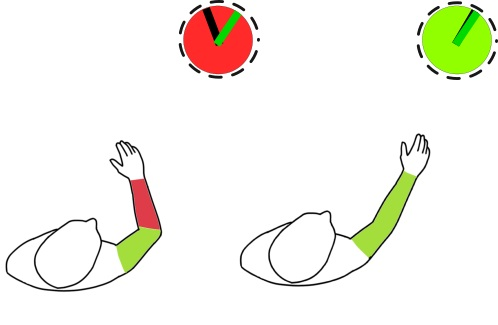
\includegraphics[width=0.8\linewidth]{imgs/approach/fullarmfeedback}
    \caption{Full Arm Visual Feedback.}
    \label{fig:fullarmfeedback}
    \endminipage\hfill
\minipage[t]{0.49\textwidth}
  \centering
  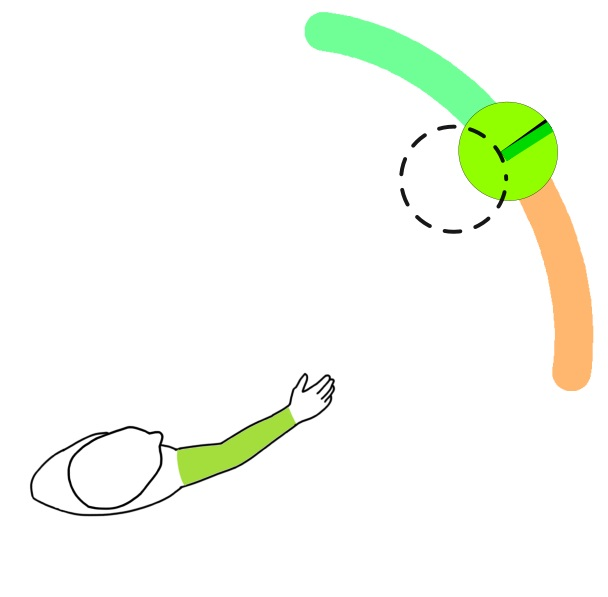
\includegraphics[width=0.8\linewidth]{imgs/approach/movementguidancefeedback}
    \caption{Movement Visual Feedback.}
    \label{fig:movementguidancefeedback}
    \endminipage
\end{figure}

Each of the previously presented designs are able to guide each arm region individually.
Hence, to guide a user to a full arm position, we combined both of them as seen on fig \ref{fig:fullarmfeedback}. 
By replacing the grey circle, used on the upper arm's design, with the elbow angle circle from the fore arm's design, we are able to use both of them simultaneously. 

All these designs are able to guide the user to a specific, but static, position. For us to be able to guide a user throughout a movement, there needs to be some changes on it.

In addition to the already presented feedback, which will be projected on the floor, we will also project information on top of the user's arm. 
In this case, we will not provide as detailed feedback as it is being provided on the floor. 
Instead, we will project different colors in each arm region depending on how far they are from the desired state. 
Once again, looking at figures \ref{fig:forearmfeedback}, \ref{fig:upperarmfeedback} and \ref{fig:fullarmfeedback}, we can observe the 
different arm regions having different colours on top, depending on the user's arm position.
These arm color projections will help in highlighting what the user might be doing incorrectly without losing focus on the main feedback.

\subsubsection{Movement Guidance}
\label{sec:movementguidance}

It is not realistic to assume that both the upper and fore arm relative position will remain static during an arm movement. 
For instance, in some movements the arm remains fully extended throughout the movement, whereas in others the fore arm may vary during the movement.  
In this latter case there is an elbow angle variation, which means the fore arm desired state is continuously changing.
With this dynamic goal in mind, our planned feedback must then change its desired state during the movement.

As for the upper arm, to help the user know where to move it, a path will be drawn showing the direction for the desired arm movement.
If we look closely at the previously presented design, we can observe it actually focus around the circle. 
The fore arm changes the circle itself, while the upper arm controls the dotted circumference that must cover also the circle. 
With this in mind, if we move this same circle through the movement path, we will be able to continuously inform the user about the 
desired direction while also updating what specific elbow angle he should have. 
In fig \ref{fig:movementguidancefeedback} we can see an example where the user is already in the middle of the exercise (at the trajectory midpoint).

\subsection{Audio}
\label{audio-feedback}

Audio feedback was found to be more suitable for timing and user notification contexts. 
Hence, we planned the usage of audio for notifying our users about specific events in SleeveAR.

In the Recording phase, SleeveAR had to provide a notification when it actually starts recording. 
In this case, a countdown audio clip was used to briefly prepare the user, so he could
position himself in the desired exercise initial position, before the actual recording began. 
Another notification sound was also played when the recording has stopped.
As for the Movement Guidance phase, SleeveAR notified the user whenever an exercise attempt started. 
From there, the main source of feedback was provided in visual form.